\documentclass[11pt]{article} 
\usepackage[english]{babel}
\usepackage[utf8]{inputenc}
\usepackage[margin=0.5in]{geometry}
\usepackage{amsmath}
\usepackage{amsthm}
\usepackage{amsfonts}
\usepackage{amssymb}
\usepackage[usenames,dvipsnames]{xcolor}
\usepackage{graphicx}
\usepackage[siunitx]{circuitikz}
\usepackage{tikz}
\usepackage[colorinlistoftodos, color=orange!50]{todonotes}
\usepackage{hyperref} 
\usepackage[numbers, square]{natbib}
\usepackage{fancybox}
\usepackage{epsfig}
\usepackage{soul}
\usepackage[framemethod=tikz]{mdframed}
\usepackage[shortlabels]{enumitem}
\usepackage[version=4]{mhchem}
\usepackage{multicol}

\usepackage{mathtools}
\usepackage{comment}
\usepackage{enumitem}
\usepackage[utf8]{inputenc}
\usepackage[linesnumbered,ruled,vlined]{algorithm2e}
\usepackage{listings}
\usepackage{color}
\usepackage[numbers]{natbib}
\usepackage{subfiles}
% \usepackage{tkz-berge}


\newtheorem{prop}{Proposition}[section]
\newtheorem{thm}{Theorem}[section]
\newtheorem{lemma}{Lemma}[section]
\newtheorem{cor}{Corollary}[prop]

\theoremstyle{definition}
\newtheorem{definition}{Definition}

\theoremstyle{definition}
\newtheorem{required}{Problem}

\theoremstyle{definition}
\newtheorem{ex}{Example}


\setlength{\marginparwidth}{3.4cm}
%#########################################################

%To use symbols for footnotes
\renewcommand*{\thefootnote}{\fnsymbol{footnote}}
%To change footnotes back to numbers uncomment the following line
%\renewcommand*{\thefootnote}{\arabic{footnote}}

% Enable this command to adjust line spacing for inline math equations.
% \everymath{\displaystyle}

% _______ _____ _______ _      ______ 
%|__   __|_   _|__   __| |    |  ____|
%   | |    | |    | |  | |    | |__   
%   | |    | |    | |  | |    |  __|  
%   | |   _| |_   | |  | |____| |____ 
%   |_|  |_____|  |_|  |______|______|
%%%%%%%%%%%%%%%%%%%%%%%%%%%%%%%%%%%%%%%

\title{
\normalfont \normalsize 
\textsc{CSCI 3104 Spring 2022 \\ 
Instructor: Profs. Chen and Layer} \\
[10pt] 
\rule{\linewidth}{0.5pt} \\[6pt] 
\huge Quiz 5 - BFS/DFS \\
\rule{\linewidth}{2pt}  \\[10pt]
}
%\author{Your Name}
\date{}

\begin{document}
\definecolor {processblue}{cmyk}{0.96,0,0,0}
\definecolor{processred}{rgb}{200, 0, 0}
\definecolor{processgreen}{rgb}{0, 255, 0}
\maketitle


%%%%%%%%%%%%%%%%%%%%%%%%%
%%%%%%%%%%%%%%%%%%%%%%%%%%
%%%%%%%%%%FILL IN YOUR NAME%%%%%%%
%%%%%%%%%%AND STUDENT ID%%%%%%%%
%%%%%%%%%%%%%%%%%%%%%%%%%%
\noindent
Due Date \dotfill February 11 \\
Name \dotfill \textbf{Chengming Li} \\
Student ID \dotfill \textbf{109251991} \\


\tableofcontents

\section{Instructions}
 \begin{itemize}
	\item The solutions \textbf{should be typed}, using proper mathematical notation. We cannot accept hand-written solutions. \href{http://ece.uprm.edu/~caceros/latex/introduction.pdf}{Here's a short intro to \LaTeX.}
	\item You should submit your work through the \textbf{class Canvas page} only. Please submit one PDF file, compiled using this \LaTeX \ template.
	\item You may not need a full page for your solutions; pagebreaks are there to help Gradescope automatically find where each problem is. Even if you do not attempt every problem, please submit this document with no fewer pages than the blank template (or Gradescope has issues with it).

	\item You \textbf{may not collaborate with other students}. \textbf{Copying from any source is an Honor Code violation. Furthermore, all submissions must be in your own words and reflect your understanding of the material.} If there is any confusion about this policy, it is your responsibility to clarify before the due date. 

	\item Posting to \textbf{any} service including, but not limited to Chegg, Discord, Reddit, StackExchange, etc., for help on an assignment is a violation of the Honor Code.

	\item You \textbf{must} virtually sign the Honor Code (see Section \ref{HonorCode}). Failure to do so will result in your assignment not being graded.
\end{itemize}


\section{Honor Code (Make Sure to Virtually Sign)} \label{HonorCode}

\begin{required}
\begin{itemize}
\item My submission is in my own words and reflects my understanding of the material.
\item Any collaborations and external sources have been clearly cited in this document.
\item I have not posted to external services including, but not limited to Chegg, Reddit, StackExchange, etc.
\item I have neither copied nor provided others solutions they can copy.
\end{itemize}

%\noindent In the specified region below, clearly indicate that you have upheld the Honor Code. Then type your name. 
\end{required}

\begin{proof}[Agreed (signature here).]
%% Typing "I agree to the above," followed by your name is sufficient.
\end{proof}


\newpage
\section{Standard 5- BFS/DFS}

\subsection{Problem \ref{dfs1}}
\begin{required} \label{dfs1}

Consider the following graph with the source node $s$:
	
\begin{center}
\noindent 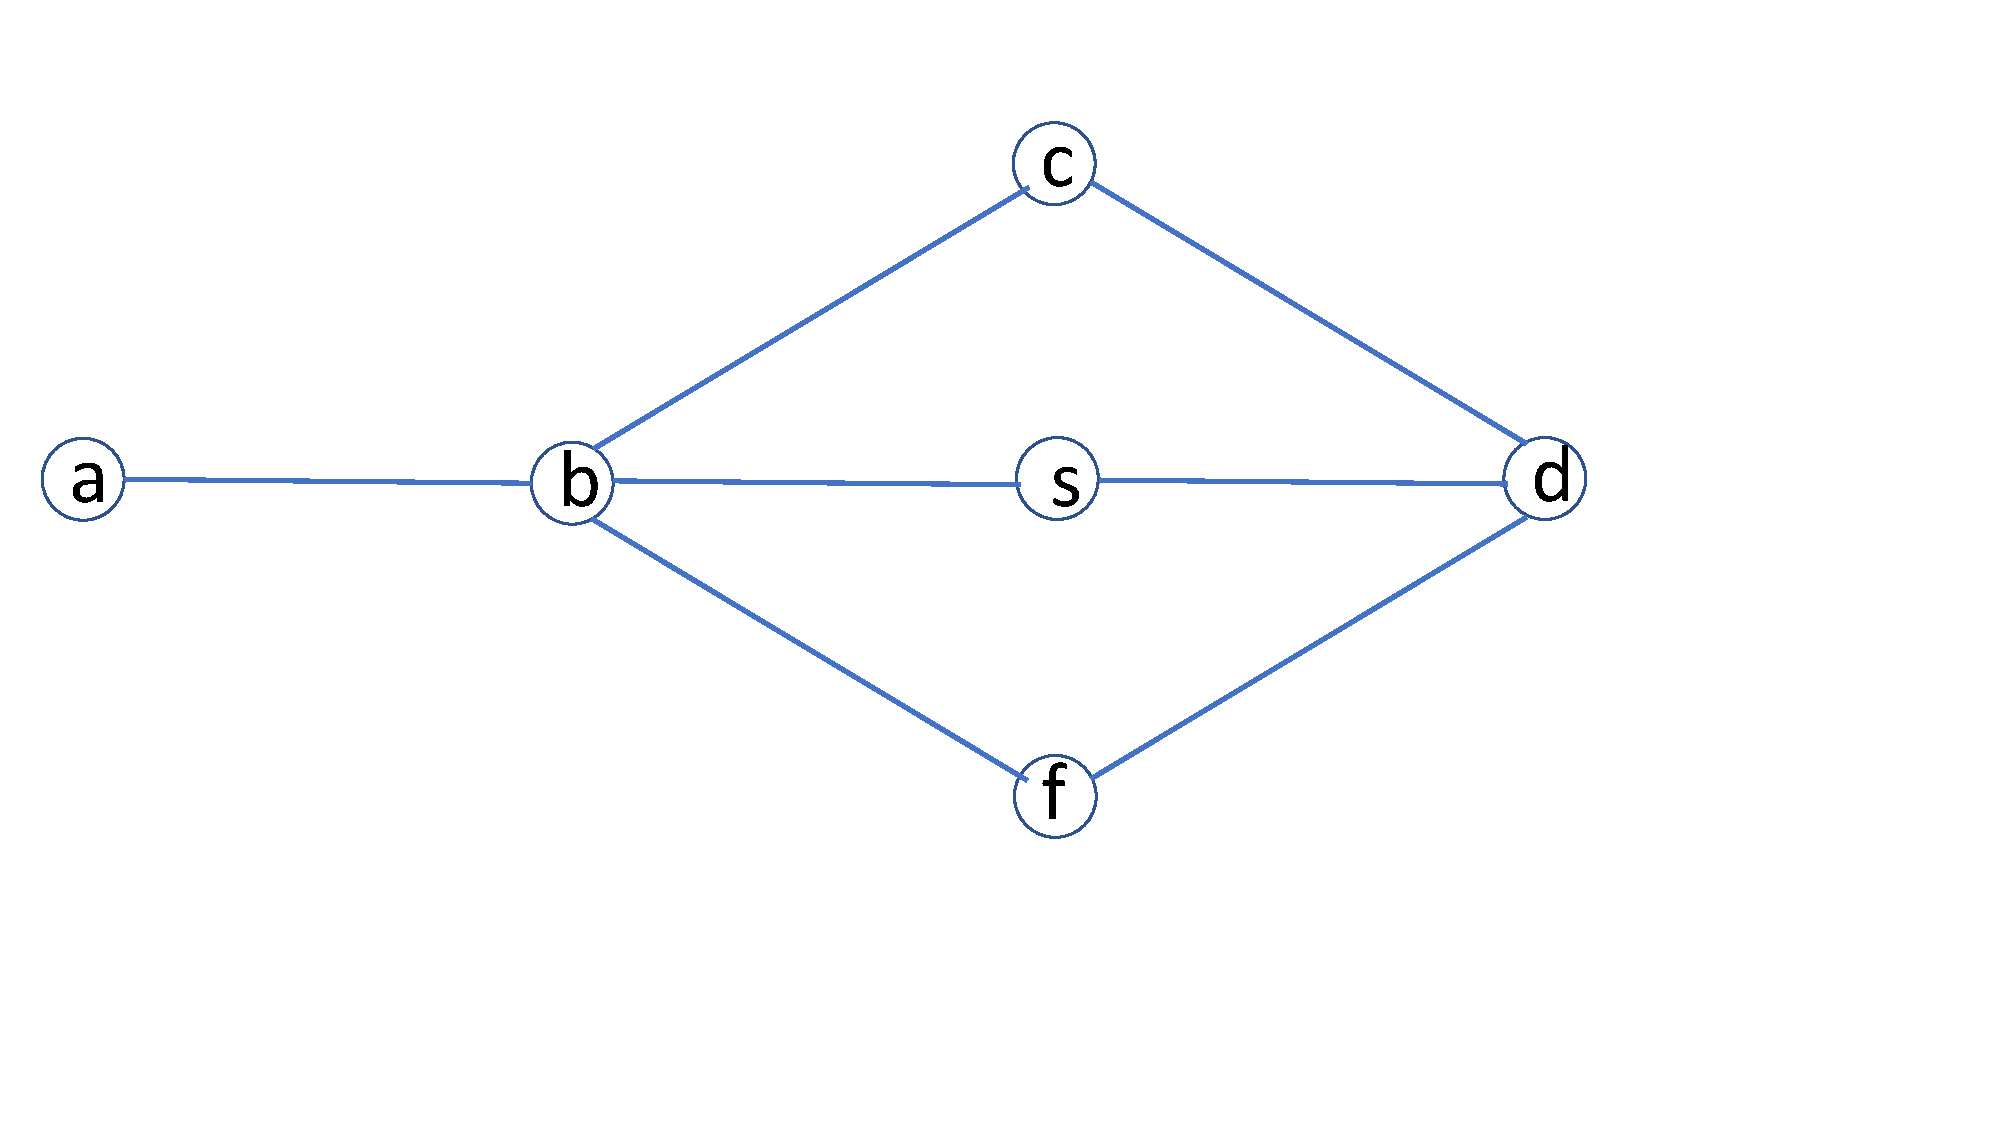
\includegraphics[scale=0.25]{BFS.pdf}
\end{center}


	(i).~Is it possible to obtain the following tree using BFS? Clearly justify your answer.
	
	
	\begin{center}
\noindent 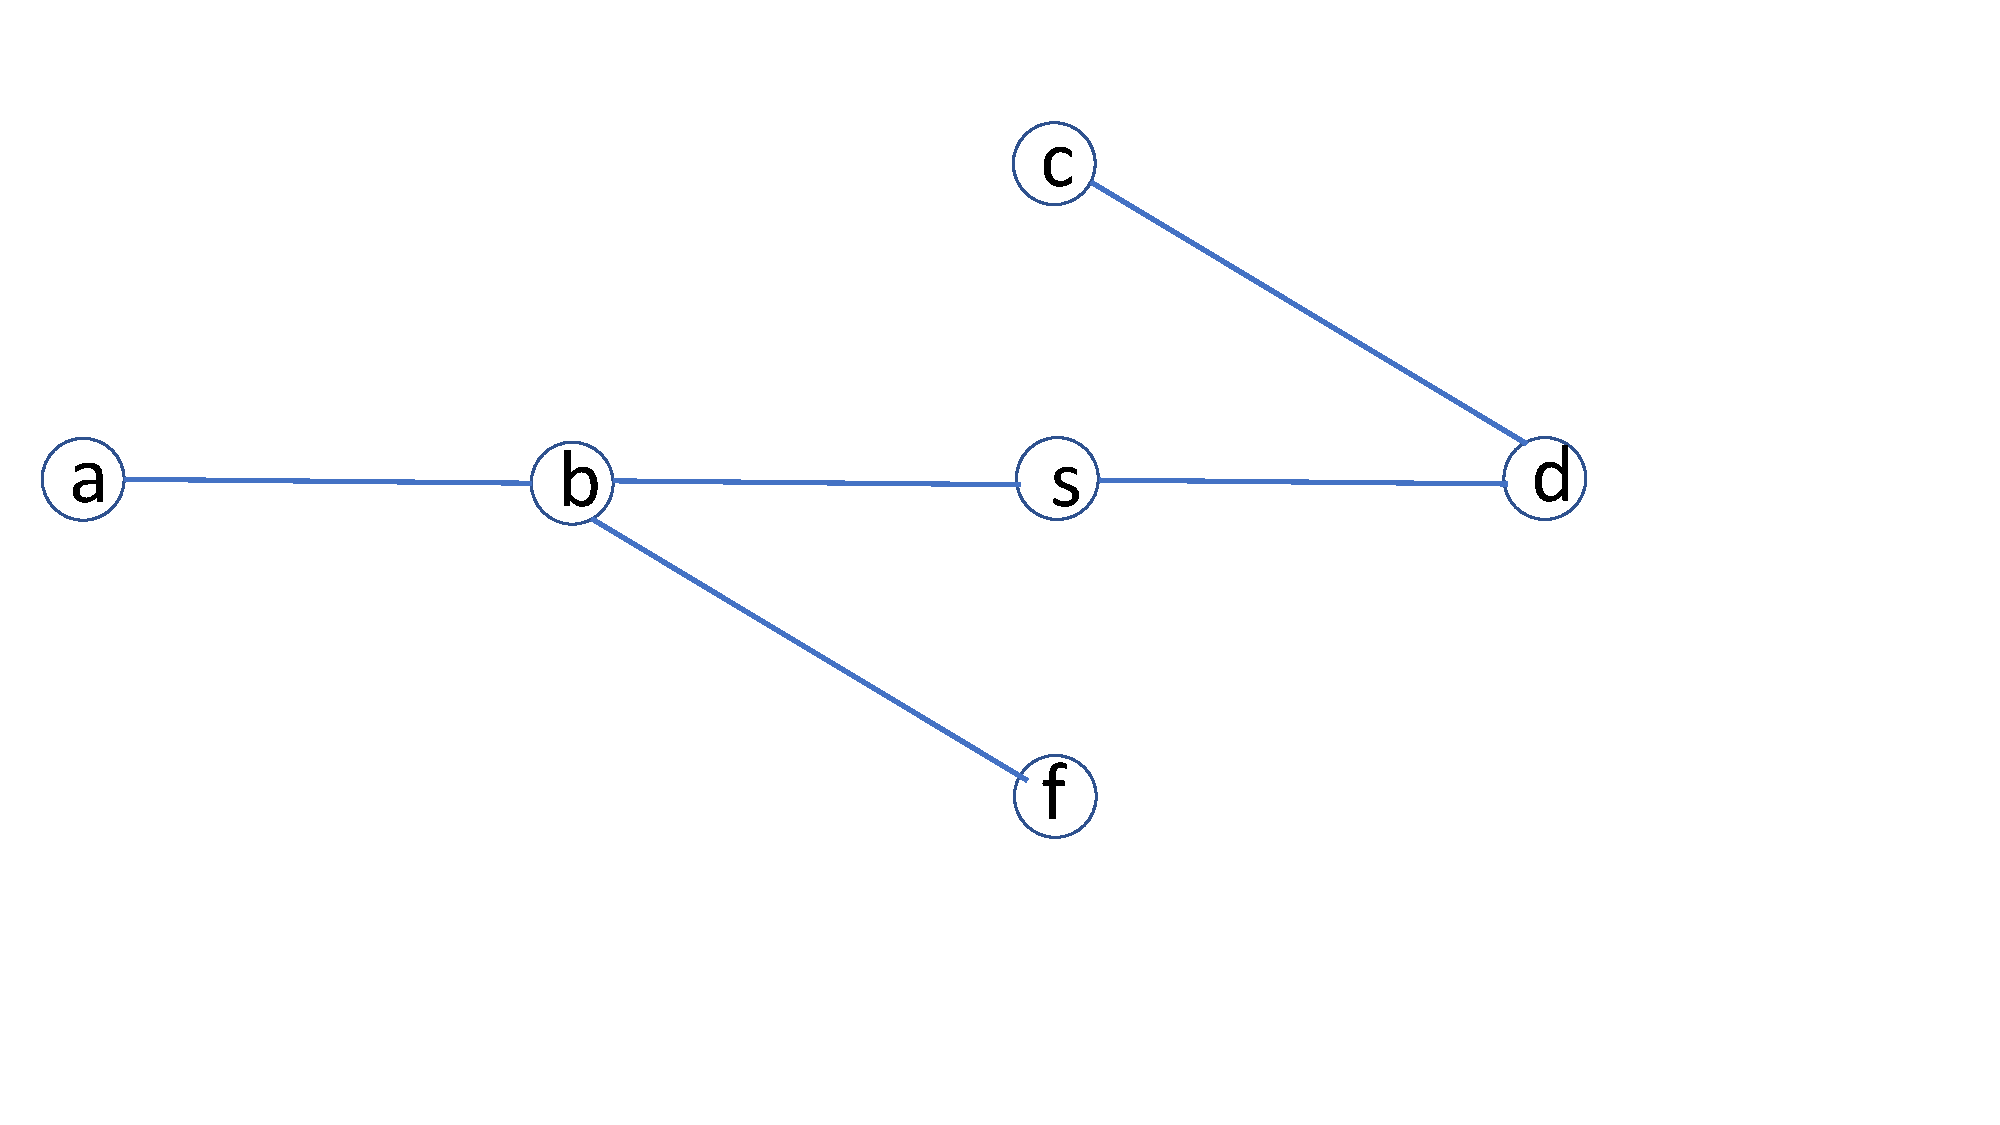
\includegraphics[scale=0.25]{tree.pdf}
\end{center}

 (ii).~Is it possible to obtain a shortest path tree using BFS? Clearly justify your answer; and if your answer is yes, give such a shortest path tree obtained using BFS. Here the length of a path is defined as the number of edges on the path. 
 
\end{required}


% Either type your answer in below, or uncomment the \includegraphics command
% and use it to insert an approprate image. Try experimenting with the scale 
% 0.9 the width option to resize your image if necessary.

%\includegraphics[width=0.9\textwidth]{solution.jpg}

\begin{proof}[Answer]
\textbf{Part I}
\begin{itemize}
\item It is impossible to obtain the tree shown in above. In the BFS algorithm, it examines all of the unvisited neighbors of the current vertex before examning vertices further. 
\item One of the possibility: content in priority queue is Q = [s]
\item Q = [b,d]
\item Q = [d,a,c,f]
\item Q = [a,c,f]
\item Q = [c,f]
\item Q = [f]
\item Q = [] Algorithm terminates
\item If we poll b before d from queue (d is already in queue), all remaining nodes, a, c and f, will be added into Q. Then, b is connected to a,c and f at the same time.
\item If we poll d before b from queue (b is already in queue), c and f will be added into queue. Then d is connected to c and f at the same time.
\item Thus, there is no way to have the tree  shown in above, like d connect to c and b connect f. Because, BFS will visit all of the unvisited neighbors of the current vertex before examing vertices further. Either b or d must connect node c and node f at the same time.
\end{itemize}
\textbf{Part II }
\begin{itemize}
\item YES, the graph is unweighted, undirected and fixed source node at s. And, BFS algorithm will visit every unvisited node that in the  same depth in tree. And the result of BFS will result in single-source shortest path trees. In other words, for any vertex v in the Graph, the s to v path in T is a shortest s to v path in G.\\
\item The shortest path from s to b or d is 1 and shortest path from s to a,c and f is 2.\\
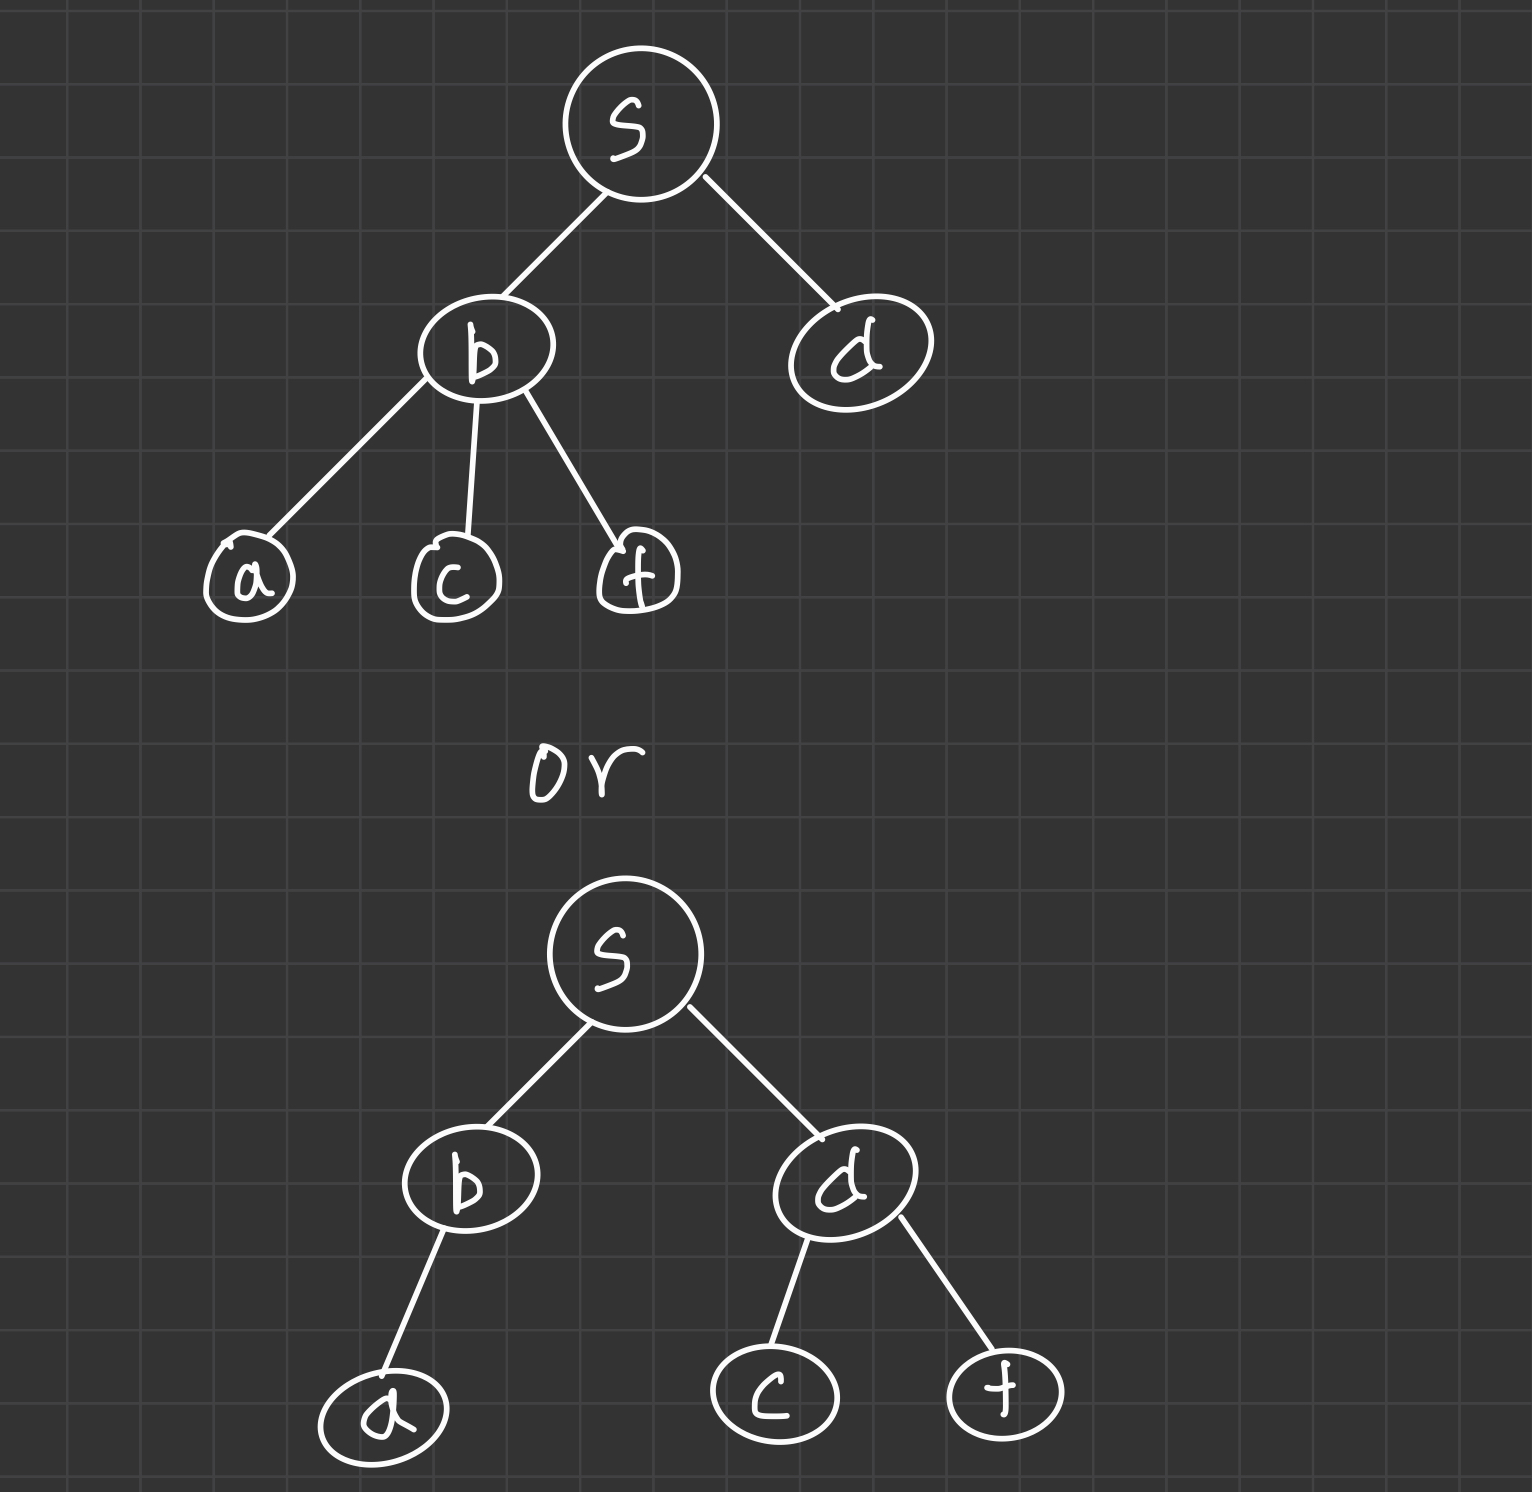
\includegraphics[width=0.7\textwidth]{S5.PNG}
\end{itemize}
\end{proof}


%Include an Image: \includegraphics{ImageFileName}
%Include an Image and Rotate 90 degree: \includegraphics[angle=90]{ImageFileName}
%Include an Image, Rotate by 180 degrees, and scale by 50\% \includegraphics[scale=0.5, angle=90]{ImageFileName}


%%%%%%%%%%%%%%%%%%%%%%%%%%%%%%%%%%%%%%%%%%%%%%%%%%
\end{document} % NOTHING AFTER THIS LINE IS PART OF THE DOCUMENT



